% Created 2017-03-11 Sat 13:16
% Intended LaTeX compiler: pdflatex
\documentclass[10pt,aspectratio=1610]{beamer}
\usepackage[utf8]{inputenc}
\usepackage[T1]{fontenc}
\usepackage{graphicx}
\usepackage{grffile}
\usepackage{longtable}
\usepackage{wrapfig}
\usepackage{rotating}
\usepackage[normalem]{ulem}
\usepackage{amsmath}
\usepackage{textcomp}
\usepackage{amssymb}
\usepackage{capt-of}
\usepackage{hyperref}
\usepackage[english]{babel}\usepackage{etex}\usepackage{minted}\usemintedstyle{emacs}
\usepackage{tikz}\usepackage{amsmath}\usepackage[T1]{fontenc}\usepackage{lmodern}%\usepackage{arev}
\usepackage{booktabs}\usepackage[citestyle=alphabetic,bibstyle=authortitle]{biblatex}
\usepackage{pgfplots,pgfplotstable}\usetikzlibrary{pgfplots.groupplots}\usepackage[babel=true,kerning=true]{microtype}\usepackage{smartdiagram}
\addbibresource{fe.bib}
\usetikzlibrary{mindmap,trees,shapes,arrows,spy,3d,decorations.pathmorphing,pgfplots.statistics,pgfplots.dateplot}
\pgfplotsset{compat=newest}
\usetheme{DarkConsole}
\author{Mathieu Fauvel}
\date{\textit{[2017-04-26 Wed 10:30]--[2017-04-26 Wed 12:00]}}
\title{Feature Extraction}
\subtitle{GRSS Summer School}
\institute{UMR Dynafor}
\AtBeginSection[]{\begin{frame}<beamer>\frametitle{Outline}\tableofcontents[currentsection]\end{frame}}
\AtBeginSubsection[]{\begin{frame}<beamer>\frametitle{Outline}\tableofcontents[currentsubsection]\end{frame}}
\setbeamercovered{again covered={\opaqueness<1->{25}}}
\usefonttheme[onlymath]{serif}
\begin{document}

\maketitle
\begin{frame}{Outline}
\tableofcontents
\end{frame}

\section{Motivations}
\label{sec:orgf88b702}
\begin{frame}[label={sec:orgb9ef503}]{Illustration}
\begin{itemize}
\item <1-> \alert{Curse of dimensionality}: it is not possible to get enough data to cover all the observation space.
\begin{center}
\emph{High dimensional saces are mostly empty !}
\end{center}
\item <2> Multivariate data live in a lower dimensional space
\begin{center}
  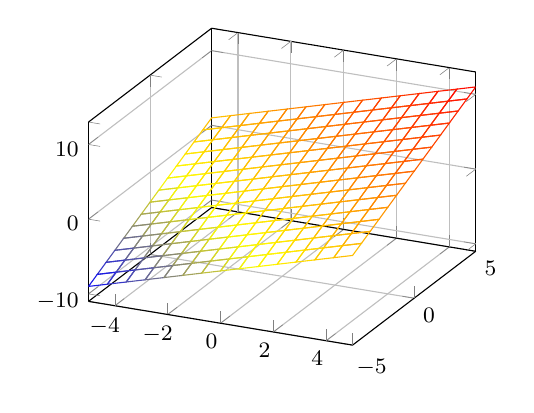
\begin{tikzpicture}
    \begin{axis}[grid=major,small]
      \addplot3 [mesh, samples=15, domain=-5:5] {x+y+1};
    \end{axis}
  \end{tikzpicture}
\end{center}
\end{itemize}
\end{frame}
\begin{frame}[label={sec:orge64b0a3}]{Application}
\begin{itemize}
\item Feature extraction is important in remote sensing because:
\begin{itemize}
\item It reduces the size of the data,
\item It limits the spatial and spectral redundancy,
\item It permits visualization of the data,
\item It mitigates the \emph{curse of dimensionality}.
\end{itemize}
\item Extraction techniques:
\begin{itemize}
\item Spectral
\begin{itemize}
\item Physically based method,
\item Statistical methods.
\end{itemize}
\item Spatial:
\begin{itemize}
\item Linear filters,
\item Non linear techniques (Mathematical Morphology)
\end{itemize}
\end{itemize}
\end{itemize}
\end{frame}


\section{Physical Indices}
\label{sec:orgc74d3a1}
\subsection{Introduction}
\label{sec:org79fae89}
\begin{frame}[label={sec:orgc5a9afc}]{Spectral indices}
\begin{itemize}
\item Spectral indices are a linear/non-linear combination of two (or more) spectral bands.
\item They provides information as a \emph{single number} about:
\begin{itemize}
\item Plant structure,
\item Biochemistry,
\item Humidity,
\item Stress.
\end{itemize}
\item Four main types \cite{hrsv:2011}:
\begin{center}
\begin{tabular}{ll}
\toprule
Name & Formulae\\
\midrule
Difference vegetation index & \(R_{\lambda_1} - R_{\lambda_2}\)\\
Ratio vegetation index & \(\dfrac{R_{\lambda_1}}{R_{\lambda_2}}\)\\
Normalized difference vegetation index & \(\dfrac{R_{\lambda_1} - R_{\lambda_2}}{R_{\lambda_1} + R_{\lambda_2}}\)\\
Soil-adjusted vegetation index & \((1+L)\times\dfrac{R_{\lambda_1} - R_{\lambda_2}}{R_{\lambda_1} - R_{\lambda_2}+L}\)\\
\bottomrule
\end{tabular}
\end{center}
\item \emph{The three last indexes are invariant to  a multiplicative factor}
\end{itemize}
\end{frame}

\begin{frame}[label={sec:org042cc7d}]{Conventional Indices}
Index database : \url{http://www.indexdatabase.de/}

\begin{center}
\small
\begin{tabular}{ll}
\toprule
Name & Formulae  (\(\lambda\) nm)\\
\midrule
Normalized Difference Vnegetation index & \(\dfrac{R_{\lambda_{800}} - R_{\lambda_{670}}}{R_{\lambda_{800}} + R_{\lambda_{670}}}\)\\
Modified Soil-Adjusted Vegetation Index & \(\dfrac{1}{2}\left[2R_{\lambda_{800}}+1 - \sqrt{(2R_{\lambda_{800}}+1)^2-8(R_{\lambda_{800}}-R_{\lambda_{670}})}\right]\)\\
Modified Chlorophyll Absorption Ratio Index & \(\left[(R_{\lambda_{700}}-R_{\lambda_{670}})-0.2(R_{\lambda_{700}}-R_{\lambda_{550}})\right]\times\dfrac{R_{\lambda_{700}}}{R_{\lambda_{670}}}\)\\
\midrule
Normalized Difference Water Index & \(\dfrac{R_{\lambda_{858}} - R_{\lambda_{1240}}}{R_{\lambda_{858}} + R_{\lambda_{1240}}}\)\\
Datt Reflectance Index & \(\dfrac{R_{\lambda_{816}} - R_{\lambda_{2218}}}{R_{\lambda_{816}} + R_{\lambda_{2218}}}\)\\
\midrule
Normalized Difference Redness Index & \(\dfrac{R_{\lambda_{540}} - R_{\lambda_{700}}}{R_{\lambda_{540}} + R_{\lambda_{700}}}\)\\
Soil Brightness Index & \(0.406R_{\lambda{550}}+0.600R_{\lambda{650}}+0.645R_{\lambda{750}}+0.243R_{\lambda{950}}\)\\
\bottomrule
\end{tabular}
\end{center}
\end{frame}

\subsection{Vegetation Indices}
\label{sec:orgee15017}
\begin{frame}[label={sec:org34b4d46}]{Normalized difference vegetation index}
$$\text{NDVI}=\dfrac{R_{\lambda_{800}} - R_{\lambda_{670}}}{R_{\lambda_{800}} + R_{\lambda_{670}}}$$
\begin{itemize}
\item \(-1\leq \text{NVDI} \leq 1\)
\item \(\text{NDVI}< 0\): surfaces other thatn plant cover
\item \(\text{NDVI}\approx 0\): bare soil
\item \(\text{NDVI}\geq 0.1\): vegetation cover (higher values correspond to more dense covers)
\end{itemize}

\begin{center}
\begin{tikzpicture}
\begin{axis}[xmin=0.4,xmax=1,ymin=0,ymax=1,grid,xlabel=$\lambda~({\mu}m)$,ylabel=Reflectance,width=0.6\linewidth,height=0.3\linewidth,cycle list name=color list]
  \addplot+[mark=none,thick,smooth] file {../Introduction/figures/oak.txt};
  \pgfplotstableread{../Introduction/figures/grass.txt}\loadedtable
  \addplot+[mark=none,smooth,thick] table[x=wave,y=grass] from \loadedtable;
  \addplot+[mark=none,smooth,thick] table[x=wave,y=drygrass] from \loadedtable;
  \pgfplotstableread{../Introduction/figures/talc.txt}\loadtable
  \addplot+[mark=none,smooth,thick] table[x=wave,y=talc] from \loadtable;
  \legend{0.81,0.90, 0.05, -0.03}
\end{axis}
\end{tikzpicture}
\end{center}
\end{frame}
\subsection{Case study}
\label{sec:orgbdc2a58}
\begin{frame}[label={sec:org8413214}]{University of Pavia}
\begin{columns}
\begin{column}{0.5\columnwidth}
\begin{center}
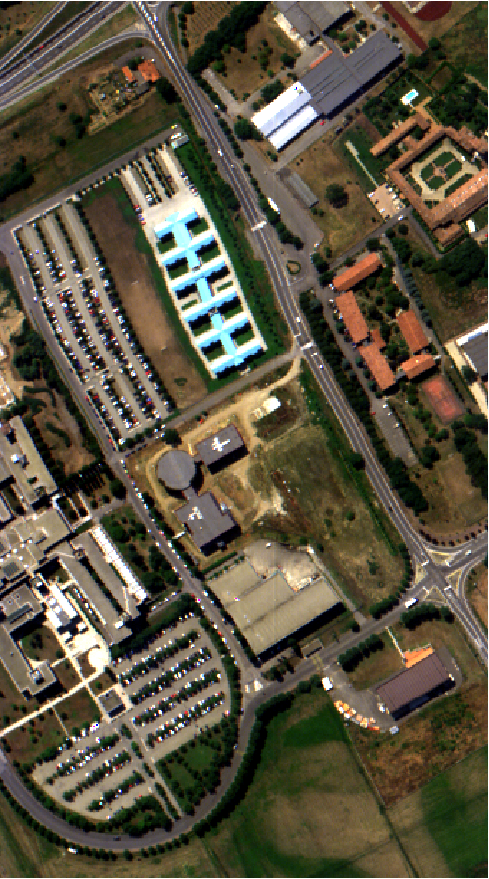
\includegraphics[width=0.6\linewidth]{./figures/university_color.png}
\end{center}
\end{column}

\begin{column}{0.5\columnwidth}
\begin{itemize}
\item Peri-urban area
\item Rosis-3 sensor
\item 103 Spectral bands (400nm-900nm)
\item 1.5 meter per pixel spatial resolution
\item 610 \(\times\) 340 pixels
\end{itemize}
\end{column}
\end{columns}
\end{frame}

\begin{frame}[fragile,label={sec:org57c4c04}]{Orfeo-Toolbox}
 \begin{itemize}
\item \href{https://www.orfeo-toolbox.org/}{OTB} is a C++ library for remote sensing images processing.
\item It is free, open-source and available for most OS (window, apple, linux)
\item \href{https://www.orfeo-toolbox.org/CookBook/OTB-Applications.html}{OTB-Applications} are set of tools appropriated for big/large images
\item They are avalaible from QGIS, Python and Bash
\item To compute the NDVI
\end{itemize}

\begin{minted}[fontsize=\footnotesize,obeytabs=true,tabsize=4,bgcolor=bg]{bash}
# Computation of the NDVI
otbcli_BandMath -il ../Data/university.tif -out ../Data/university_ndvi.tif \
		-exp "(im1b83-im1b56)/(im1b83+im1b56)"

# Computation of the SBI
otbcli_BandMath -il ../Data/university.tif -out ../Data/university_sbi.tif \
		-exp "0.406*im1b31 + 0.6*im1b52 + 0.645*im1b73"
\end{minted}
\end{frame}

\begin{frame}[label={sec:org9cefc90}]{University of Pavia - Spectral Indices}
\begin{columns}
\begin{column}{0.3\columnwidth}
\begin{center}
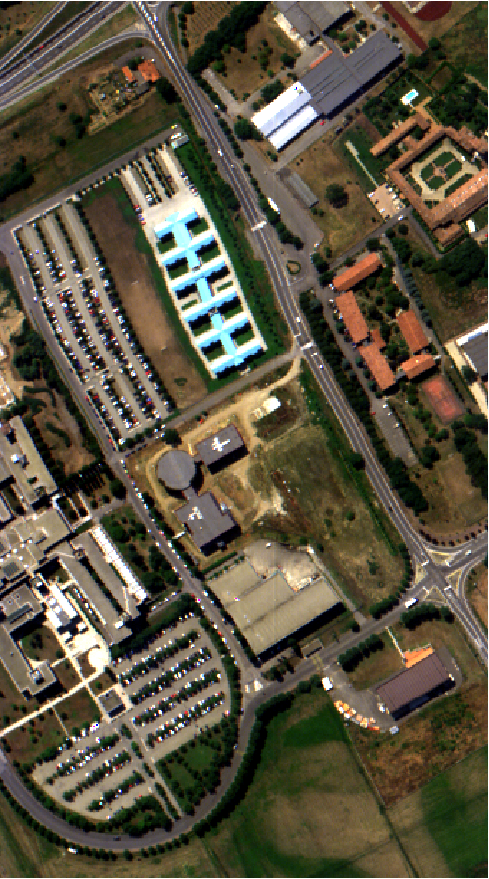
\includegraphics[width=\linewidth]{./figures/university_color.png}
\end{center}
\end{column}

\begin{column}{0.3\columnwidth}
\begin{center}
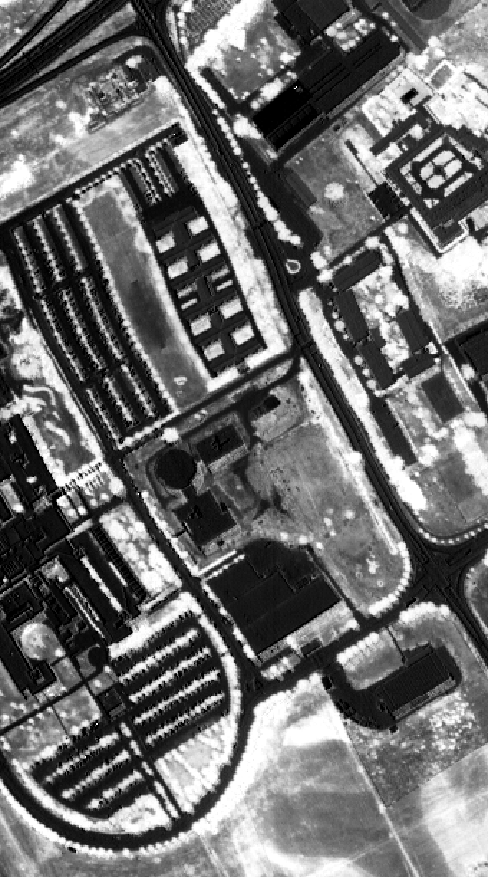
\includegraphics[width=\linewidth]{./figures/university_ndvi.png}
\end{center}
\end{column}

\begin{column}{0.3\columnwidth}
\begin{center}
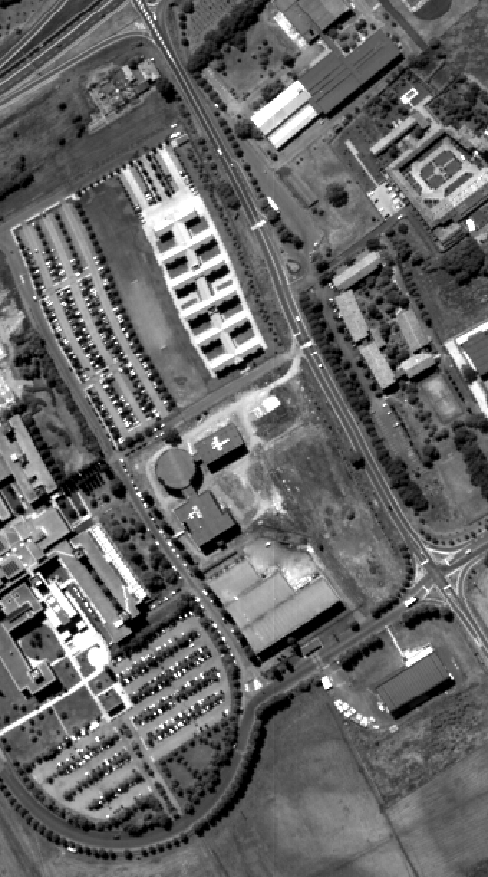
\includegraphics[width=\linewidth]{./figures/university_sbi.png}
\end{center}
\end{column}
\end{columns}
\end{frame}

\begin{frame}[fragile,label={sec:org190dc40}]{Where is the vegetation 1/2 ?}
   \begin{center}
  \begin{tikzpicture}
    \begin{axis}[grid=both,width=0.95\linewidth,height=0.45\linewidth,/pgf/number format/1000 sep={},/pgf/number format/fixed,title=Density plot of the NDVI,xmin=-0.6,xmax=1,ymin=0,ymax=0.01]
      \addplot+[mark=none,thick,smooth] table[x=x,y=y,col sep=comma] {figures/pdf.csv};
      \only<2->{\addplot[red,thick] coordinates {(0.19,0) (0.19,0.008)};
      \addplot[red,thick] coordinates {(0.62,0) (0.62,0.008)}; }     
    \end{axis}
\end{tikzpicture}
\end{center}

\begin{minted}[fontsize=\footnotesize,obeytabs=true,tabsize=4,bgcolor=bg]{bash}
# Segmentation of the NDVI in three classes
otbcli_BandMath -il ../Data/university_ndvi.tif -out ../Data/university_ndvi_segmented.tif \
		-exp "(im1b1<0.19?1:(im1b1<0.62?2:3))"
\end{minted}
\end{frame}

\begin{frame}[label={sec:orgf28b76e}]{Where is the vegetation 2/2 ?}
\begin{columns}
\begin{column}{0.5\columnwidth}
\begin{center}
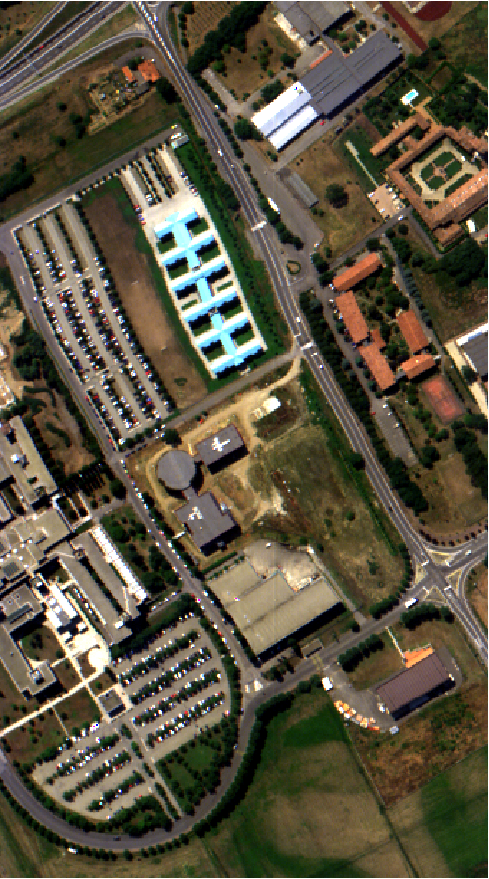
\includegraphics[width=0.6\linewidth]{./figures/university_color.png}
\end{center}
\end{column}

\begin{column}{0.5\columnwidth}
\begin{center}
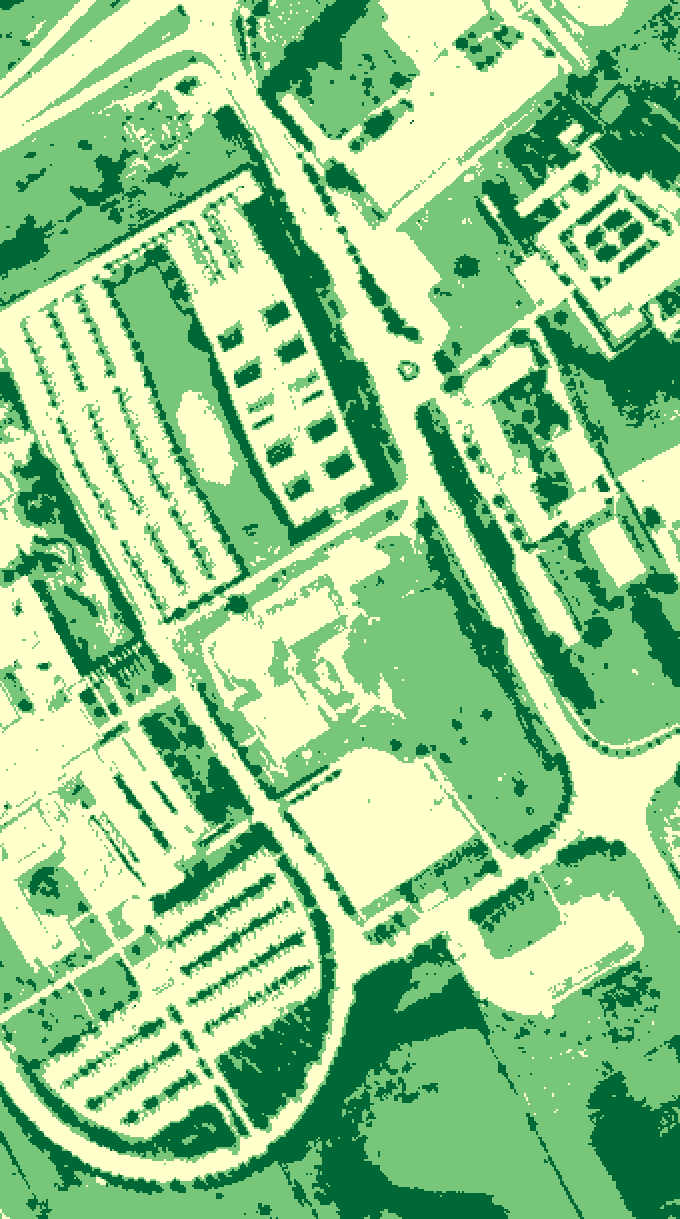
\includegraphics[width=0.6\linewidth]{./figures/university_ndvi_segmented.png}
\end{center}
\end{column}
\end{columns}
\end{frame}

\subsection{Question}
\label{sec:orgc854835}
\begin{frame}[label={sec:org314f229}]{Could you find the good one ?}
 \centerline{\begin{tabular}{cc}
    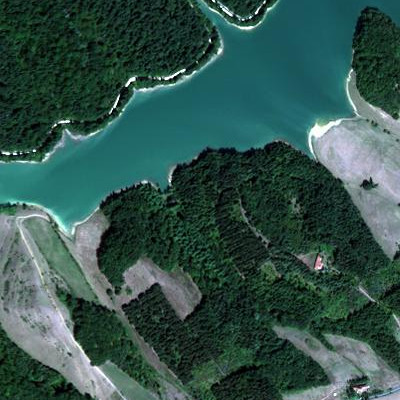
\includegraphics[width=0.4\linewidth]{figures/image1.jpg} & \begin{tikzpicture}\pgfplotsset{every axis legend/.append style={at={(0.5,1.03)},anchor=south}}
      \begin{axis}[ytick=\empty,xmin=-0.5,xmax=0.9,ymin=0,width=0.5\linewidth,axis y line=center,axis x line=bottom,legend columns=4]
        \pgfplotstableread{figures/ndvi1.txt}\loadedtable
        \addplot[smooth,very thick,dashed,blue] table[x=wave,y=ndvi] from \loadedtable;
        \pgfplotstableread{figures/ndvi2.txt}\loadedtable
        \addplot[smooth,very thick,magenta] table[x=wave,y=ndvi] from \loadedtable;
        \pgfplotstableread{figures/ndvi3.txt}\loadedtable
        \addplot[smooth,very thick,dotted,orange] table[x=wave,y=ndvi] from \loadedtable;
        \pgfplotstableread{figures/ndvi4.txt}\loadedtable
        \addplot[smooth,very thick,dashdotted,green] table[x=wave,y=ndvi] from \loadedtable;
        \legend{ndvi$_1$,ndvi$_2$,ndvi$_3$,ndvi$_4$};
      \end{axis}
    \end{tikzpicture}\\
    Image & NDVI Histogram
\end{tabular}}
\vspace{1cm}

From the histogram, which one does correspond to the NDVI of the image ?
\end{frame}
\section{Statistical Feature Extraction}
\label{sec:org18d9ab5}
\subsection{Unsupervised}
\label{sec:org4031569}
\begin{frame}[label={sec:org880e147}]{Principal Components Analysis}
\begin{itemize}
\item Linear transformation used to reduce the dimensionality of the data \cite{jolliffe2002principal}.
$$ z_i = \langle\mathbf{v}_i,\mathbf{x}\rangle$$
\item Find features \(\mathbf{z}\) that  account for most of the variability of the data:
\begin{itemize}
\item \(z_1,~z_2,~z_3,\ldots\) are mutually uncorrelated,
\item \(\text{var}(z_i)\) is as large as possible,
\item \(\text{var}(z_1)>\text{var}(z_2)>\text{var}(z_3)>\ldots\)
\end{itemize}
\end{itemize}

\begin{center}
  \begin{tikzpicture}
    \begin{axis}[grid,small,width=0.4\linewidth,height=0.32\linewidth,xmin=0,xmax=2.5,ymin=0,ymax=2]
      \addplot[only marks,blue] table[x index=0,y index = 1,col sep =comma] {figures/pca_data.csv};
      \begin{scope}
      \addplot[very thick,red] coordinates { (0.080264,0.83834891)  (2.06023219,1.12070676)};
      \addplot[very thick,red] coordinates { (0.92906917,  1.96951193)(1.21142702, -0.01045626)};
    \end{scope}

   \end{axis}                                  
  \end{tikzpicture}
\end{center}
\end{frame}
\begin{frame}[label={sec:orgbc29acd}]{Maximization of the variance 1/2}
\begin{itemize}
\item <1-> Search \(\mathbf{v}_1\) such as \(\max\text{var}(z_1)\):
\begin{eqnarray*}
  \text{var}(z_1) & = & \text{var}(\langle\mathbf{v}_1,\mathbf{x}\rangle)\\
  &=& \mathbf{v}_1^\top\boldsymbol{\Sigma}\mathbf{v}_1
\end{eqnarray*}
\item <2-> Indetermined: if \(\hat{\mathbf{v}}_1\) maximizes the variance, \(\alpha\hat{\mathbf{v}}_1\) too!  Add a constraint: \(\langle\mathbf{v}_1,\mathbf{v}_1\rangle=1\)
\item <3-> Lagrangian:
\begin{eqnarray*}
  \mathcal{L}(\mathbf{v}_1,\lambda_1) = \mathbf{v}_1^\top\boldsymbol{\Sigma}\mathbf{v}_1 + \lambda_1(1- \mathbf{v}_1^\top\mathbf{v}_1)  
\end{eqnarray*}
\item <4-> Compute the derivative w.r.t \(\mathbf{v}_1\):
\begin{eqnarray*}
\frac{\partial\mathcal{L}}{\partial\mathbf{v}_1} = 2\boldsymbol{\Sigma}\mathbf{v}_1-2\lambda_1\mathbf{v}_1
\end{eqnarray*}
\item <5-> \(\mathbf{v}_1\) is an eigenvector of the covariance matrix of \(\mathbf{x}\):
\begin{eqnarray*}
  \boldsymbol{\Sigma}\mathbf{v}_1 =\lambda_1\mathbf{v}_1
\end{eqnarray*}
\item <6->  \(\mathbf{v}_1\) is the eigenvector corresponding to the largest eigenvalues !
\begin{eqnarray*}
  \text{var}(z_1)  =  \mathbf{v}_1^\top\boldsymbol{\Sigma}\mathbf{v}_1 = \lambda_1 \mathbf{v}_1^\top\mathbf{v}_1 = \lambda_1
\end{eqnarray*}
\end{itemize}
\end{frame}
\begin{frame}[label={sec:orge7bd2f3}]{Maximization of the variance 2/2}
\begin{itemize}
\item <1-> Search \(\mathbf{v}_2\) such as \(\max\text{var}(z_2)\) and \(\langle\mathbf{v}_2,\mathbf{v}_2\rangle=1\) and \(\langle\mathbf{v}_1,\mathbf{v}_2\rangle=0\)
\item <2-> Lagrangian:
\begin{eqnarray*}
  \mathcal{L}(\mathbf{v}_2,\lambda_2,\beta_1) = \mathbf{v}_2^\top\boldsymbol{\Sigma}\mathbf{v}_2 + \lambda_1(1- \mathbf{v}_2^\top\mathbf{v}_2) + \beta_1(0 - \mathbf{v}_2^\top\mathbf{v}_1)
\end{eqnarray*}
\item <3-> Compute the derivative w.r.t \(\mathbf{v}_2\):
\begin{eqnarray*}
\frac{\partial\mathcal{L}}{\partial\mathbf{v}_2} &=& 2\boldsymbol{\Sigma}\mathbf{v}_2-2\lambda_1\mathbf{v}_2-\beta_1\mathbf{v}_1\\
\boldsymbol{\Sigma}\mathbf{v}_2 &=& \lambda_1\mathbf{v}_2+2\beta_1\mathbf{v}_1
\end{eqnarray*}
\item <4-> At optimality, \(\langle\mathbf{v}_1,\mathbf{v}_2\rangle=0\). Left-multiplying by \(\mathbf{v}_1^\top\) the above equation:
\begin{eqnarray*}
  \mathbf{v}_1^\top\boldsymbol{\Sigma}\mathbf{v}_2 &=& 2\beta_1 \\
  \lambda_1\mathbf{v}_1^\top\mathbf{v}_2 &=& 2\beta_1 \\
  0 &=& 2\beta_1 \\
\end{eqnarray*}
\item <5-> Hence, we have 
\begin{eqnarray*}
  \boldsymbol{\Sigma}\mathbf{v}_2 =\lambda_2\mathbf{v}_2
\end{eqnarray*}
\item <6-> \(\mathbf{v}_2\) is the eigenvector corresponding the \emph{second largest} eigenvalues
\item <7-> \(\mathbf{v}_k\) is the eigenvector corresponding the \emph{\(k^{\text{th}}\) largest} eigenvalues
\end{itemize}
\end{frame}
\begin{frame}[label={sec:org2856e27}]{PCA in practice}
\begin{enumerate}
\item Empirical estimation the mean value:
\begin{eqnarray*}
  \boldsymbol{\mu} = \frac{1}{n}\sum_{i=1}^n\mathbf{x}_i
\end{eqnarray*}
\item Empirical estimation the covariance matrix:
\begin{eqnarray*}
  \boldsymbol{\Sigma} = \frac{1}{n-1}\sum_{i=1}^n(\mathbf{x}_i-\boldsymbol{\mu})(\mathbf{x}_i-\boldsymbol{\mu})^\top
\end{eqnarray*}
\item Compute \(p\) first eigenvalues/eigenvectors\ldots{} How to choose \(p\) ? Explained variance: 
$$\frac{\sum_{i=1}^p\lambda_i}{\sum_{i=1}^d\lambda_i}$$
\item Tips for high dimensional data set: if \(n<d\) see \cite{manolakis2016hyperspectral} page 420
\end{enumerate}
\end{frame}
\begin{frame}[fragile,label={sec:org1edab08}]{PCA case study 1/3}
 \begin{minted}[fontsize=\footnotesize,obeytabs=true,tabsize=4,bgcolor=bg]{python}
import rasterTools as rt
import scipy as sp
from sklearn.decomposition import PCA
import matplotlib.pyplot as plt

# Load data set
im,GeoT,Proj = rt.open_data('../Data/university.tif')
[h,w,b]=im.shape
im.shape=(h*w,b)
wave = sp.loadtxt('../Data/waves.csv',delimiter=',')

# Do PCA
pca = PCA()
pca.fit(im)

# Plot explained variance
l = pca.explained_variance_ratio_
print l[:5]
print (l.cumsum()/l.sum())[:5]

# Save Eigenvectors
D = sp.concatenate((wave[:,sp.newaxis],pca.components_[:3,:].T),axis=1)
sp.savetxt('../FeatureExtraction/figures/pca_pcs.csv',D,delimiter=',')
\end{minted}
\end{frame}
\begin{frame}[label={sec:orgf5e56dc}]{PCA case study 2/3}
\begin{itemize}
\item Explained variance
\begin{center}
  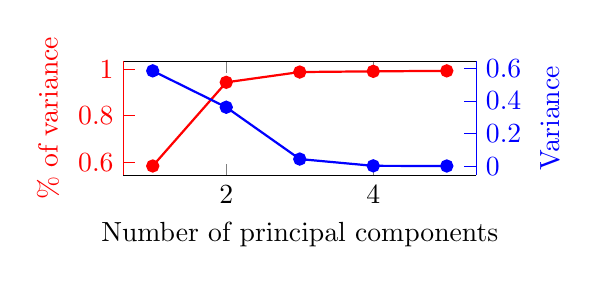
\begin{tikzpicture}
    \begin{axis}[width=0.5\textwidth,height=0.25\textwidth,ylabel=\% of variance,xlabel=Number of principal components,axis y line*=left,yticklabel style=red,ylabel style=red, y axis line style=red,ytick style=red]
      \addplot[thick,mark=*,red] coordinates { (1,0.58318064)  (2,0.94418758)  (3,0.98856319)  (4,0.99157161)  (5,0.99366953)};
    \end{axis}
    \begin{axis}[width=0.5\textwidth,height=0.25\textwidth,axis y line*=right,axis x line=none,ylabel=Variance,yticklabel style=blue,ylabel style=blue, y axis line style=blue,ytick style=blue]
      \addplot[thick,mark=*,blue] coordinates { (1,0.58318064)  (2,0.36100695)  (3,0.04437561)  (4,0.00300841)  (5,0.00209792)};
    \end{axis}
  \end{tikzpicture}
\end{center}
\item Principal components
\begin{center}
  \begin{tikzpicture}
    \begin{axis}[width=0.9\textwidth,height=0.3\textwidth,grid,xmin=400,xmax=900,cycle list name=color list]
      \addplot+[thick] table[col sep=comma,x index=0,y index=1] {figures/pca_pcs.csv};
      \addplot+[thick] table[col sep=comma,x index=0,y index=2] {figures/pca_pcs.csv};
      \addplot+[thick] table[col sep=comma,x index=0,y index=3] {figures/pca_pcs.csv};
      \legend{pc1,pc2,pc3};
    \end{axis}
  \end{tikzpicture}
\end{center}
\end{itemize}
\end{frame}
\begin{frame}[fragile,label={sec:orgab9d789}]{PCA case study 3/3}
 \begin{minted}[fontsize=\footnotesize,obeytabs=true,tabsize=4,bgcolor=bg]{python}
# Projection of the first PCs
imp = sp.dot(im,pca.components_[:3,:].T)
imp.shape = (h,w,3)

# Save image
rt.write_data('../Data/pca_university.tif',imp,GeoT,Proj)
\end{minted}
\begin{columns}
\begin{column}{0.3\columnwidth}
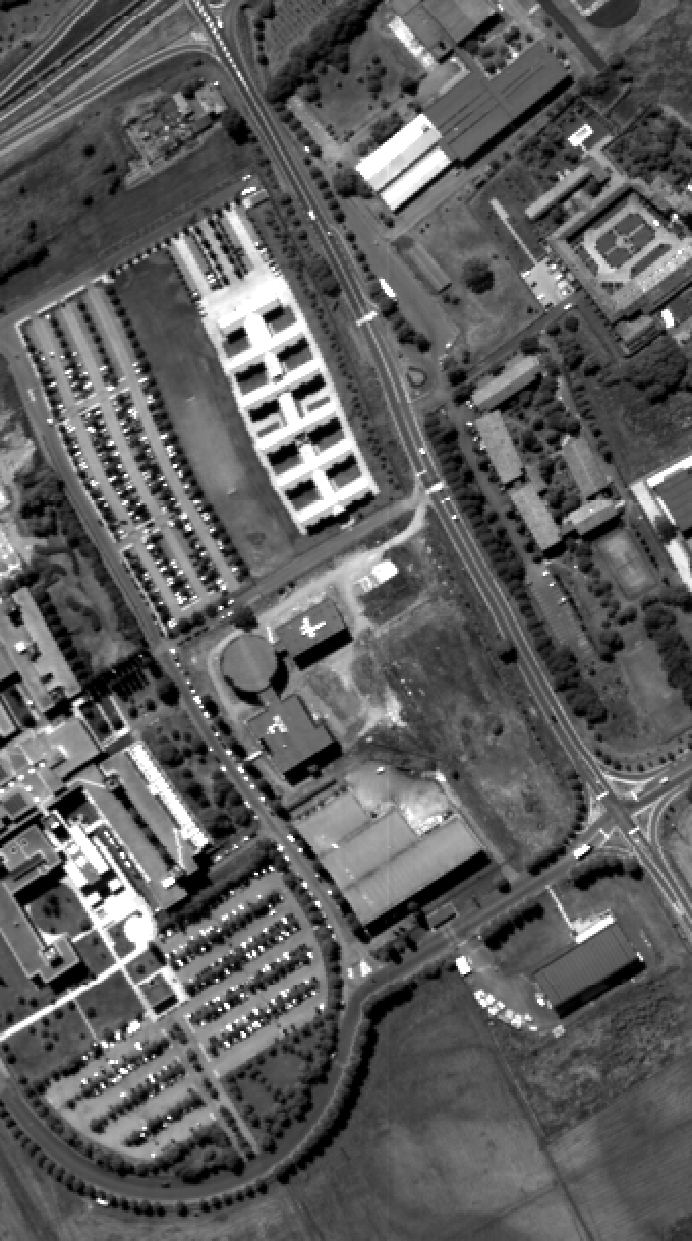
\includegraphics[width=0.75\linewidth]{./figures/university_pc1.png}
\end{column}

\begin{column}{0.3\columnwidth}
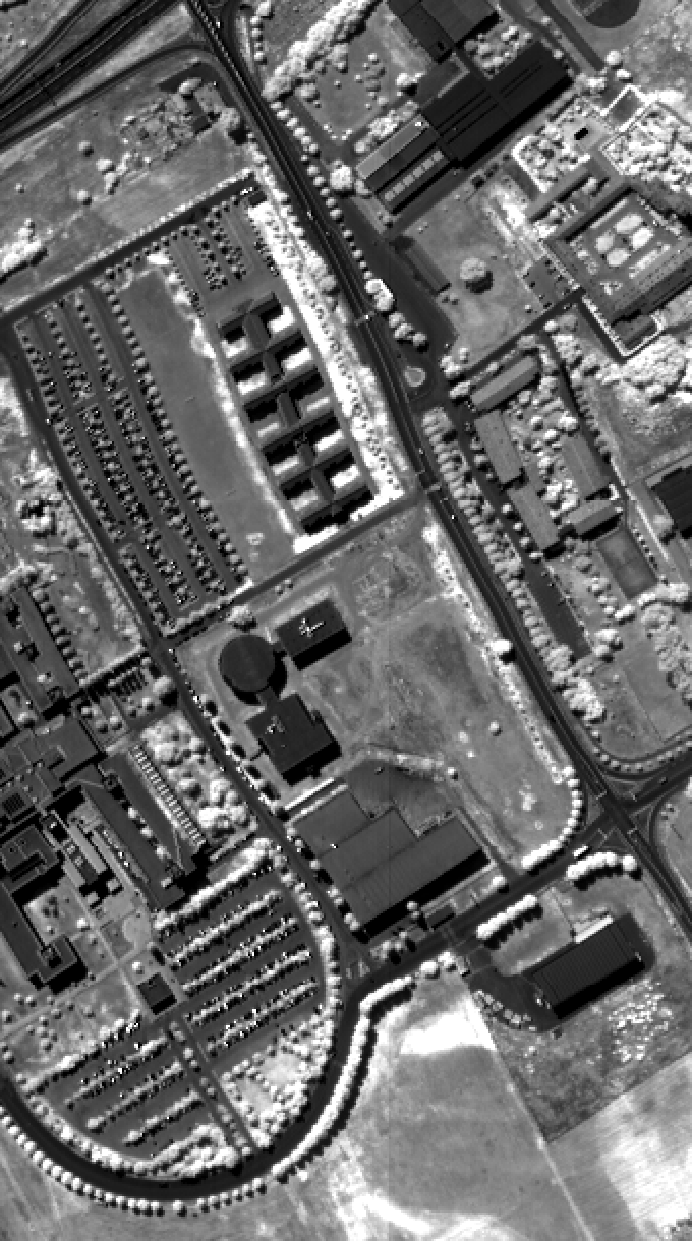
\includegraphics[width=0.75\linewidth]{./figures/university_pc2.png}
\end{column}

\begin{column}{0.3\columnwidth}
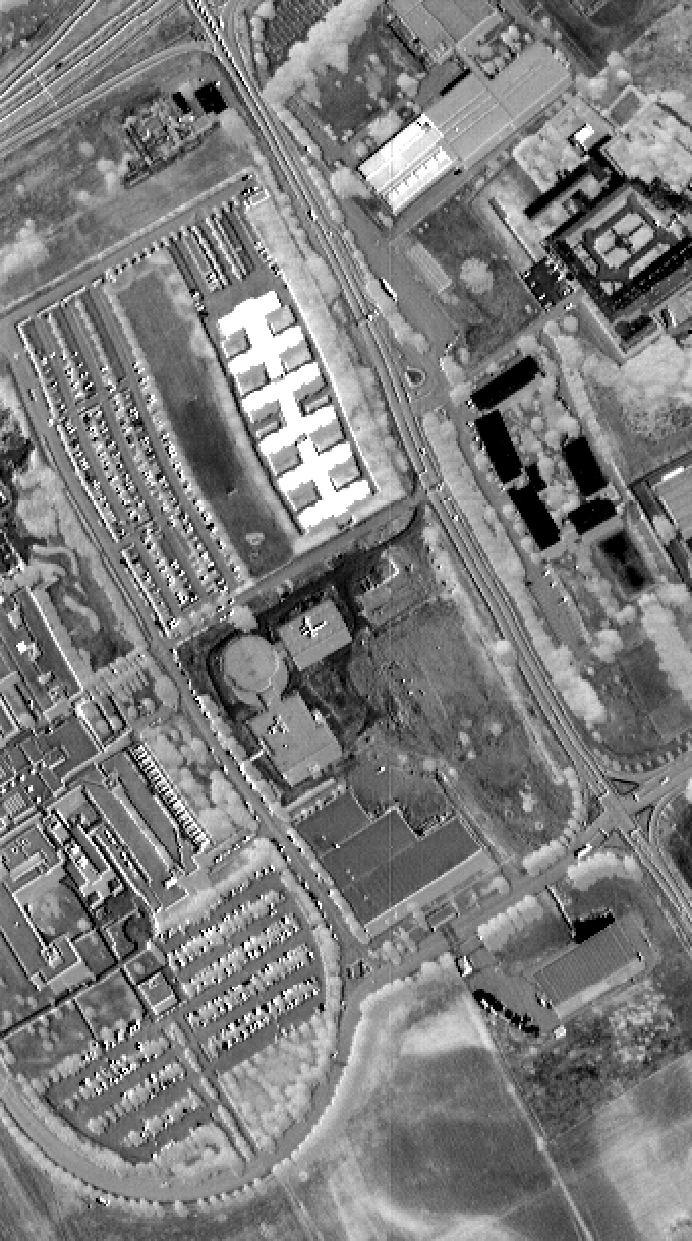
\includegraphics[width=0.75\linewidth]{./figures/university_pc3.png}
\end{column}
\end{columns}
\end{frame}

\begin{frame}[label={sec:orgb4829a4}]{Kernel PCA}
\begin{itemize}
\item PCA is limited to second order information
\item To capture higher-order statistics, it is possible to map the data onto another space \(\mathcal{H}\)
\begin{eqnarray*}
  \begin{array}{rcl}
    \phi:\mathbb{R}^d &\to&\mathcal{H}\\
    \mathbf{x}&\mapsto&\phi(\mathbf{x}).
  \end{array}
\end{eqnarray*}
\item In \(\mathcal{H}\), conventional PCA can be applied.
\item Using the \emph{kernel trick} it is possible to directly work on the \emph{kernel matrix} in \(\mathbb{R}^d\)
\begin{eqnarray*}\label{kpca:matrix}
 \mathbf{K}=\left(
 \begin{array}{cccc}
 k(\mathbf{x}_1,\mathbf{x}_1) & k(\mathbf{x}_1,\mathbf{x}_2) & \ldots & k(\mathbf{x}_1,\mathbf{x}_n)\\
 k(\mathbf{x}_2,\mathbf{x}_1) & k(\mathbf{x}_2,\mathbf{x}_2) & \ldots & k(\mathbf{x}_2,\mathbf{x}_n)\\ 
 \vdots & \vdots & \ddots & \vdots \\
 k(\mathbf{x}_n,\mathbf{x}_1) & k(\mathbf{x}_n,\mathbf{x}_2) & \ldots & k(\mathbf{x}_n,\mathbf{x}_n)\\
 \end{array}\right).
\end{eqnarray*}
\item <2> KPCA versus PCA:

\begin{center}
  \begin{tabular}{ccc}
  \begin{tikzpicture}
    \begin{axis}[width=0.3\textwidth,height=0.3\textwidth,grid]
      \addplot[scatter,only marks,scatter src=explicit] table[col sep =comma,meta index=2,x index=0,y index=1] {figures/kpca_data.csv};
    \end{axis}
  \end{tikzpicture}&
  \begin{tikzpicture}
    \begin{axis}[width=0.3\textwidth,height=0.3\textwidth,grid]
      \addplot[scatter,only marks,scatter src=explicit] table[col sep =comma,meta index=2,x index=0,y index=1] {figures/kpca_datap.csv};
    \end{axis}
  \end{tikzpicture}&
                     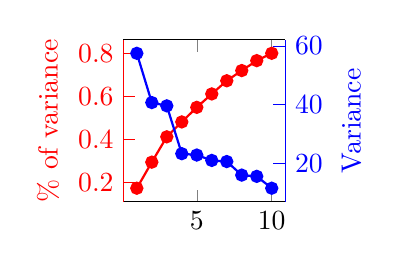
\begin{tikzpicture}
      \begin{axis}[width=0.3\textwidth,height=0.3\textwidth,ylabel=\% of variance,axis y line*=left,yticklabel style=red,ylabel style=red, y axis line style=red,ytick style=red]
        \addplot[thick,mark=*,red] coordinates { (1,0.171950045779)
          (2,0.293633371022)
          (3,0.41194893578)
          (4,0.481444806977)
          (5,0.54956124474)
          (6,0.612183510855)
          (7,0.673659036749)
          (8,0.721296411495)
          (9,0.767653893262)
          (10,0.80191080235)};
      \end{axis}
      \begin{axis}[width=0.3\textwidth,height=0.3\textwidth,axis y line*=right,axis x line=none,ylabel=Variance,yticklabel style=blue,ylabel style=blue, y axis line style=blue,ytick style=blue]
        \addplot[thick,mark=*,blue] coordinates {(1,57.4446834929)
          (2,40.6516908637)
          (3,39.5265970358)
          (4,23.2170239146)
          (5,22.7561859043)
          (6,20.9207054308)
          (7,20.5376050443)
          (8,15.914586718)
          (9,15.4870029584)
          (10,11.4444709279) };
      \end{axis}
    \end{tikzpicture}         
  \end{tabular}

\end{center}
\end{itemize}
\end{frame}

\begin{frame}[label={sec:org66f0a4b}]{Kernel PCA in practice}
\begin{itemize}
\item Choose the kernel and its parameters
\item Compute the kernel matrix \(\mathbf{K}\) for all the pixels (or a subset)
\item Center the matrix
\begin{eqnarray*}
 \mathbf{K}_c=\mathbf{K}-\mathbf{1}_n\mathbf{K}-\mathbf{K}\mathbf{1}_n+\mathbf{1}_n\mathbf{K}\mathbf{1}_n
\end{eqnarray*}
\item Solve the eigenproblems
\begin{eqnarray*}
  \lambda\boldsymbol{\alpha}=\mathbf{K}\boldsymbol{\alpha} \text{ subject to } \|\boldsymbol{\alpha}\|_2 = \frac{1}{\lambda}
\end{eqnarray*}
\item Project on the \(p\) first \emph{kernel principal components}: \(\phi^{kpc}(\mathbf{x})=\begin{bmatrix}\phi^{kpc}_1(\mathbf{x})&\hdots&\phi^{kpc}_p(\mathbf{x})\end{bmatrix}^t\)
\begin{eqnarray*}
  \phi^{kpc}_j(\mathbf{x})=\sum_{i=1}^n \alpha_{ki} k(\mathbf{x}_i,\mathbf{x})
\end{eqnarray*}
\end{itemize}
\end{frame}

\begin{frame}[fragile,label={sec:org2f8d4e2}]{KPCA case study 1/3}
 \begin{minted}[fontsize=\footnotesize,obeytabs=true,tabsize=4,bgcolor=bg]{python}
import rasterTools as rt
import scipy as sp
from sklearn.decomposition import KernelPCA
import matplotlib.pyplot as plt
from sklearn.preprocessing import StandardScaler

# Load data set
im,GeoT,Proj = rt.open_data('../Data/university.tif')
[h,w,b]=im.shape
im.shape=(h*w,b)
wave = sp.loadtxt('../Data/waves.csv',delimiter=',')

# Scale data
sc = StandardScaler()
im = sc.fit_transform(im)

# Do KPCA
kpca = KernelPCA(kernel='rbf',gamma=1.0/b,n_jobs=-1)
kpca.fit(im[::50,:]) # Use a subset of the total pixel number
\end{minted}
\end{frame}
\begin{frame}[label={sec:orgef06dc6}]{KPCA case study 2/3}
\begin{itemize}
\item Explained variance
\begin{center}
  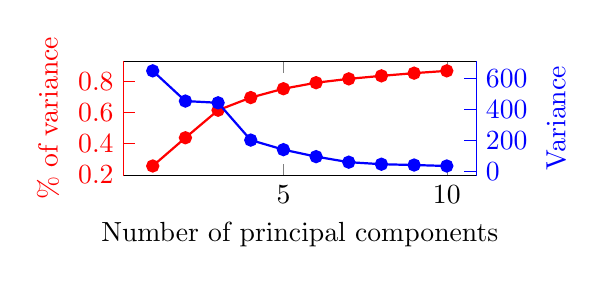
\begin{tikzpicture}
    \begin{axis}[width=0.5\textwidth,height=0.25\textwidth,ylabel=\% of variance,xlabel=Number of principal components,axis y line*=left,yticklabel style=red,ylabel style=red, y axis line style=red,ytick style=red]
      \addplot[thick,mark=*,red] coordinates {(1,0.257631571125)
      (2,0.438129567049)
      (3,0.61420975716)
      (4,0.695091757082)
      (5,0.751533118467)
      (6,0.790148033382)
      (7,0.814644462352)
      (8,0.833924207631)
      (9,0.851128186791)
      (10,0.865878267501) };
    \end{axis}
    \begin{axis}[width=0.5\textwidth,height=0.25\textwidth,axis y line*=right,axis x line=none,ylabel=Variance,yticklabel style=blue,ylabel style=blue, y axis line style=blue,ytick style=blue]
      \addplot[thick,mark=*,blue] coordinates {(1,649.766197024)
      (2,455.229519695)
      (3,444.087481204)
      (4,203.990486367)
      (5,142.349357966)
      (6,97.389719371)
      (7,61.7818360658)
      (8,48.6249674864)
      (9,43.3897292304)
      (10,37.2008127987) };
      \end{axis}
  \end{tikzpicture}
\end{center}
\item Principal components
\begin{center}
  \begin{tikzpicture}
    \begin{axis}[width=0.9\textwidth,height=0.3\textwidth,grid,cycle list name=color list,xmin=0,xmax=4148]
      \addplot+[thick] table[col sep=comma,x index=0,y index=1] {figures/kpca_pcs.csv};
      \addplot+[thick] table[col sep=comma,x index=0,y index=2] {figures/kpca_pcs.csv};
      \addplot+[thick] table[col sep=comma,x index=0,y index=3] {figures/kpca_pcs.csv};
      \legend{kpc1,kpc2,kpc3};
    \end{axis}
  \end{tikzpicture}
\end{center}
\end{itemize}
\end{frame}
\begin{frame}[fragile,label={sec:orga380b9d}]{KPCA case study 3/3}
 \begin{minted}[fontsize=\footnotesize,obeytabs=true,tabsize=4,bgcolor=bg]{python}
imp = kpca.transform(im)[:,:3]
imp.shape = (h,w,3)

# Save image
rt.write_data('../Data/kpca_university.tif',imp,GeoT,Proj)
\end{minted}
\begin{columns}
\begin{column}{0.3\columnwidth}
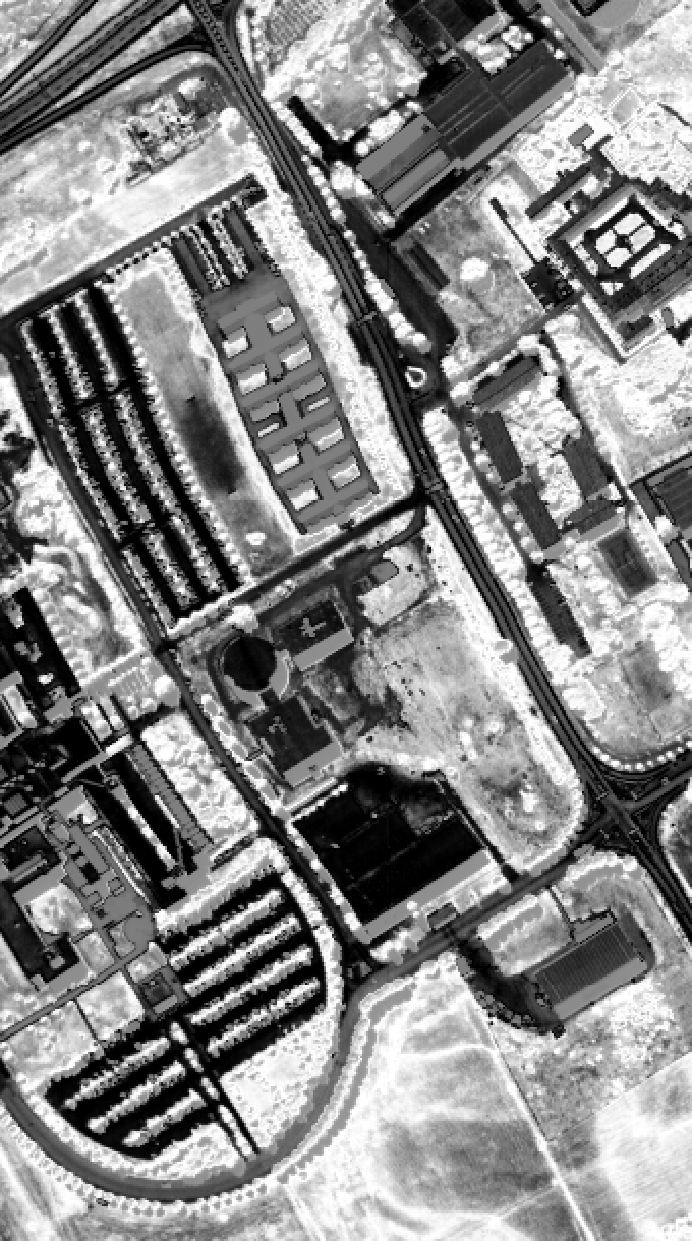
\includegraphics[width=0.75\linewidth]{./figures/university_kpc1.png}
\end{column}

\begin{column}{0.3\columnwidth}
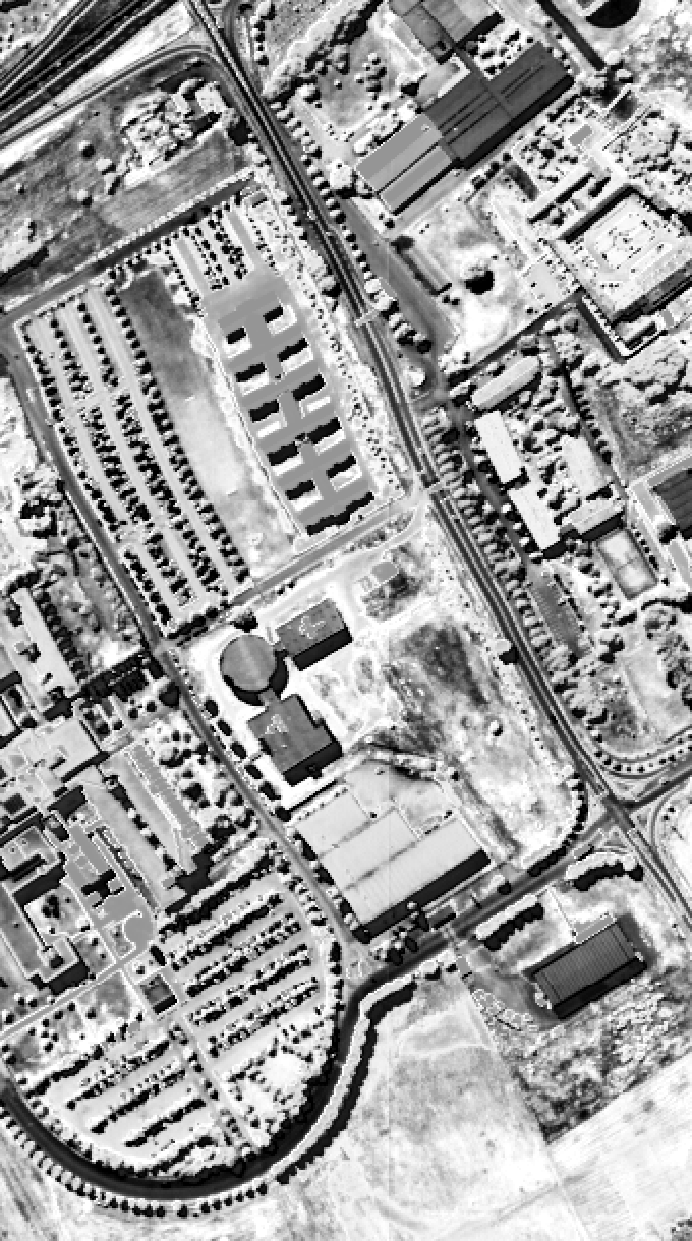
\includegraphics[width=0.75\linewidth]{./figures/university_kpc2.png}
\end{column}

\begin{column}{0.3\columnwidth}
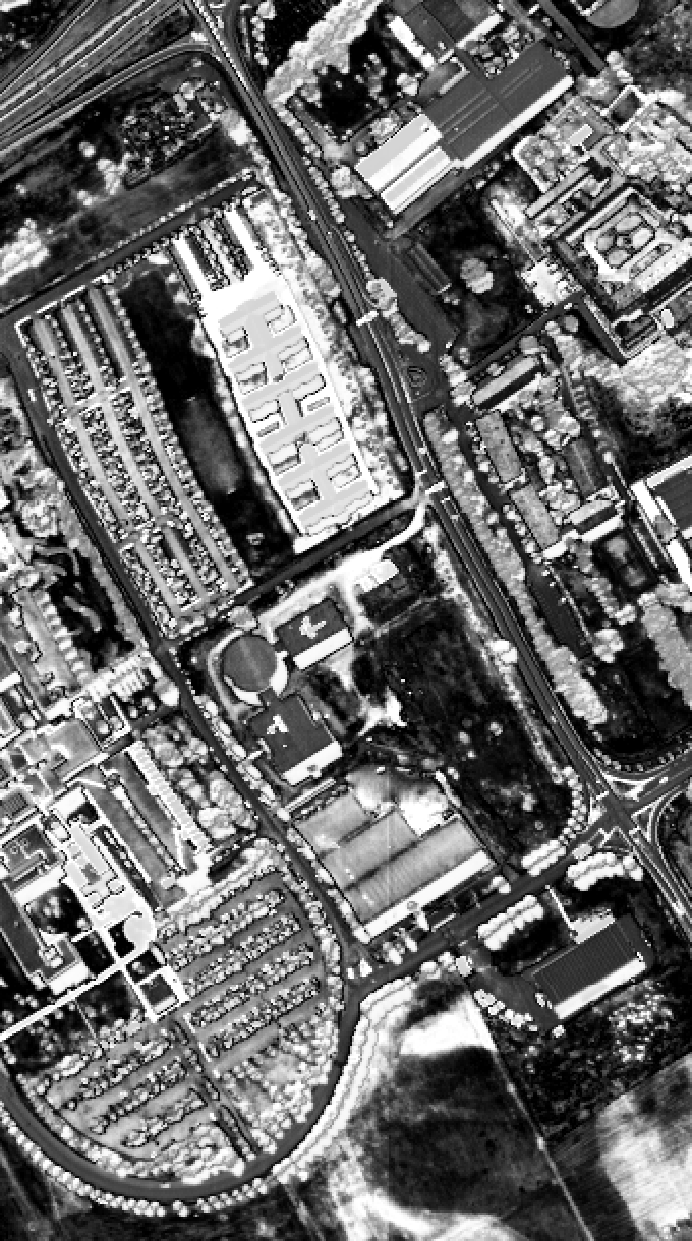
\includegraphics[width=0.75\linewidth]{./figures/university_kpc3.png}
\end{column}
\end{columns}
\end{frame}

\subsection{Supervised}
\label{sec:org9c68c9a}
\end{document}